\chapter{Results and Discussion}

%% English draft. \crosscheck{...} flags values a human must re-verify against the FINAL
%% run before submission. All numbers below are the current experimental values.

This chapter first summarises the realised system. It then reports the results of each
evaluation tier defined in Chapter~III: graph construction quality, guideline concordance
and the observation-gate ablation, manual gold-standard validation, safety detection,
briefing faithfulness, and the clinician review. It closes with a comparison against prior
work and a discussion. Every tier is automated except the clinician review, whose coverage is
limited, as set out in Section~\ref{sec:limitations}.

Each section answers a specific research objective from Section~1.3.
Table~\ref{tab:ro-map} states the correspondence explicitly.

\begin{table}[h]
\centering
\caption{Mapping of research objectives to the sections that answer them.}
\label{tab:ro-map}
\begin{tabular}{@{}p{96mm}p{46mm}@{}}
\hline
\textbf{Research objective} & \textbf{Answered in} \\
\hline
RO1 -- FHIR-native pipeline, knowledge graph, concept bridge, and end-to-end evaluation
    & Sections \ref{sec:sys-impl}, \ref{sec:kg-results}, \ref{sec:gold},
      \ref{sec:safety-detection}, \ref{sec:clinician} \\
RO2 -- Observation gates and the concordance ablation
    & Section \ref{sec:ablation} \\
RO3 -- Grounded briefing and its faithfulness
    & Section \ref{sec:faithfulness} \\
\hline
\end{tabular}
\end{table}

\section{System Implementation}
\label{sec:sys-impl}

The design of Chapter~III was realised as a set of Python programs operating on a Neo4j
knowledge graph. The principal components are:

\begin{itemize}
    \item a \textbf{FHIR-to-Neo4j loader} that maps each FHIR resource to a node, each
    reference to a relationship typed after the element it came from
    (\texttt{Observation.subject} yields a \texttt{SUBJECT} edge, not a generic one), and
    each terminology code to a shared \texttt{:Code}
    node, with multi-valued observations expanded into component nodes and an observation
    allow-list applied; all writes are idempotent (\texttt{MERGE}), so re-loading is safe;
    \item a \textbf{terminology bridge} that exports the graph's EHR codes and maps them to
    UMLS concepts via a three-pass linker (exact alias, candidate generation, then
    NLP-based linking), producing the \texttt{SAME\_CONCEPT} spine;
    \item \textbf{guideline and literature layers} that attach the curated recommendations
    and the guideline-seeded literature corpus onto the shared concept nodes;
    \item a \textbf{recommendation query layer} (applicable recommendations, observation
    gates, contraindication safety, and literature-PMI ranking); and
    \item a \textbf{grounded-briefing pipeline} that deterministically retrieves the
    recommendation facts and has a large language model phrase them, followed by an
    automated faithfulness check.
\end{itemize}

Table~\ref{tab:modules} lists the implementation modules and their functions. The system is
implemented in Python, with Cypher for the graph-construction steps, against a Neo4j
database; the knowledge graph is built once and then queried per patient.

\begin{table}[h]
\centering
\caption{Implementation modules and their functions.}
\label{tab:modules}
\begin{tabular}{@{}p{42mm}p{100mm}@{}}
\hline
\textbf{Module} & \textbf{Function} \\
\hline
Loader\newline{\scriptsize \texttt{loader.py}} & Load FHIR R4 bundles into Neo4j (nodes, edges, shared \texttt{:Code} nodes) \\
Code export\newline{\scriptsize \texttt{graph\_export\_ehr\_codes.py}} & Export the deduplicated EHR codes from the graph for bridging \\
UMLS bridge\newline{\scriptsize \texttt{snomed\_umls\_bridge.py}} & Map EHR codes to UMLS CUIs (three-pass linker) \\
Concept layer\newline{\scriptsize \texttt{ehr\_concept\_kg.cypher}} & Create concepts and \texttt{SAME\_CONCEPT} edges to \texttt{:Code} nodes \\
Guideline layer\newline{\scriptsize \texttt{guideline\_kg.cypher}} & Load recommendations, COR-derived edges, and citations \\
Literature layer\newline{\scriptsize \texttt{literature\_kg.cypher}} & Load abstracts, entity mentions, and PMI co-occurrence edges \\
Observation gates\newline{\scriptsize \texttt{obs\_gate.py}} & Decide observation-dependent recommendations from graph features \\
NSAID chronicity\newline{\scriptsize \texttt{nsaid\_csv.py}} & Compute chronic-NSAID status from CSV course durations \\
Recommendation / evaluation\newline{\scriptsize \texttt{crs\_eval.py}, \texttt{eval\_by\_class.py}} & Applicable-set, safety, and literature queries; concordance scoring \\
Reference standard (oracle)\newline{\scriptsize \texttt{silver\_oracle.py}} & CRS-independent labels read from the raw FHIR bundles \\
Grounded briefing\newline{\scriptsize \texttt{crs\_briefing.py}} & Deterministic retrieval + LLM phrasing \\
Faithfulness check\newline{\scriptsize \texttt{faithfulness\_check.py}} & Verify the briefing against the retrieved facts \\
\hline
\end{tabular}
\end{table}

Each module is named beside its source file. Appendix~\ref{app:modules} lists the
supporting scripts alongside them and reproduces three listings that carry the design
decisions the text turns on: the loader's idempotent \texttt{MERGE}, the
observation-gate predicate, and the briefing prompt.

Figure~\ref{fig:architecture} places the modules of Table~\ref{tab:modules} in the
designed system. The language model sits at the end of the chain and receives only what
deterministic retrieval has already assembled. The reference standard is computed from the
raw record rather than from the knowledge graph that was built.

\begin{figure}[htbp]
\centering
\resizebox{\textwidth}{!}{%
\begin{tikzpicture}[
    node distance = 9mm and 3mm,
    box/.style   = {rectangle, rounded corners=2pt, draw, text width=22mm,
                    align=center, minimum height=11mm, font=\scriptsize},
    src/.style   = {box, fill=black!5},
    store/.style = {rectangle, rounded corners=2pt, draw, very thick, fill=black!12,
                    text width=129.5mm, align=center, minimum height=12mm, font=\scriptsize},
    pay/.style   = {rectangle, rounded corners=2pt, draw, dashed,
                    text width=129.5mm, align=center, minimum height=9mm, font=\scriptsize},
    ev/.style    = {box, fill=black!8},
    fn/.style    = {font=\tiny},
    band/.style  = {font=\scriptsize\itshape, inner sep=0pt},
    ar/.style    = {-latex, thick},
    raw/.style   = {-latex, dashed}
]
\node[src] (s1) {Synthea FHIR R4 bundles\\[1pt]\emph{5{,}490 patients}};
\node[src, right=of s1] (s2) {Synthea CSV export\\[1pt]\emph{start/stop dates}};
\node[src, right=of s2] (s3) {UMLS Metathesaurus};
\node[src, right=of s3] (s4) {PubMed abstracts\\[1pt]\emph{4{,}801, guideline-seeded}};
\node[src, right=of s4] (s5) {2023 AHA/ACC CCD guideline};

\node[box, below=of s1] (b1) {EHR layer\\[1pt]{\fn\texttt{loader.py}}};
\node[box, right=of b1] (b2) {Code export\\[1pt]{\fn\texttt{graph\_export\_}\\\texttt{ehr\_codes.py}}};
\node[box, right=of b2] (b3) {UMLS bridge\\[1pt]{\fn\texttt{snomed\_umls\_}\\\texttt{bridge.py}}};
\node[box, right=of b3] (b4) {Concept and literature layers\\[1pt]{\fn\texttt{ehr\_concept\_kg}\\\texttt{literature\_kg}\\(\texttt{.cypher})}};
\node[box, right=of b4] (b5) {Guideline layer\\[1pt]{\fn\texttt{guideline\_kg}\\\texttt{.cypher}}};

\node[store, below=9mm of b3] (store)
    {\textbf{\texttt{sihdfhir}} (Neo4j)\\[1pt]
     EHR $\cdot$ concept $\cdot$ guideline $\cdot$ literature layers\\[1pt]
     \emph{1{,}804{,}379 nodes, 8{,}796{,}425 relationships}};

\node[box, below=9mm of store.south west, anchor=north west] (v1)
    {Applicable set\\[1pt]\emph{CCD gate, then AND/OR}};
\node[box, right=of v1] (v2) {Observation gate\\[1pt]{\fn\texttt{obs\_gate.py}}};
\node[box, right=of v2] (v3) {Safety flags\\[1pt]\emph{contraindications}};
\node[box, right=of v3] (v4) {Literature support\\[1pt]\emph{PMI ranking}};
\node[box, right=of v4] (v5) {NSAID chronicity\\[1pt]{\fn\texttt{nsaid\_csv.py}}};

\node[pay, below=9mm of v3] (facts)
    {Facts payload\\[1pt]\emph{every item carries its recommendation id, COR and PMIDs}};

\node[box, below=9mm of facts.south west, anchor=north west] (p1)
    {Language model\\[1pt]\emph{phrasing only}};
\node[box, right=of p1] (p2) {Briefing\\[1pt]\emph{main + details}};
\node[box, right=of p2] (p3) {Faithfulness check\\[1pt]{\fn\texttt{faithfulness\_}\\\texttt{check.py}}};

\node[ev, below=9mm of p1] (e1)
    {Reference standard\\[1pt]{\fn\texttt{silver\_oracle.py}}};
\node[ev, right=of e1] (e2)
    {Concordance and ablation\\[1pt]{\fn\texttt{crs\_eval.py}\\\texttt{eval\_by\_class.py}}};

\node[band, anchor=south west] at ([yshift=1mm]s1.north west) {Sources};
\node[band, anchor=south west] at ([yshift=1mm]b1.north west) {Build, run once};
\node[band, anchor=south west] at ([yshift=1mm]v1.north west) {Per patient};
\node[band, anchor=south west] at ([yshift=1mm]e1.north west) {Evaluation};

% sources into the build
\draw[ar] (s1) -- (b1);
\draw[ar] (s3) -- (b3);
\draw[ar] (s4) -- (b3);
\draw[ar] (s5) -- (b5);

% build writes the store; the code export reads it back
\draw[ar] (b1) -- (store.north -| b1);
\draw[ar] (store.north -| b2) -- (b2);
\draw[ar] (b2) -- (b3);
\draw[ar] (b3) -- (b4);
\draw[ar] (b4) -- (store.north -| b4);
\draw[ar] (b5) -- (store.north -| b5);

% every per-patient query reads the same store
\draw[ar] (store.south -| v1) -- (v1);
\draw[ar] (store.south -| v2) -- (v2);
\draw[ar] (store.south -| v3) -- (v3);
\draw[ar] (store.south -| v4) -- (v4);
\draw[ar] (store.south -| v5) -- (v5);

% retrieval assembles the payload; the model only phrases it
\draw[ar] (v1) -- (facts.north -| v1);
\draw[ar] (v2) -- (facts.north -| v2);
\draw[ar] (v3) -- (facts.north -| v3);
\draw[ar] (v4) -- (facts.north -| v4);
\draw[ar] (v5) -- (facts.north -| v5);
\draw[ar] (facts.south -| p1) -- (p1);
\draw[ar] (p1) -- (p2);
\draw[ar] (p2) -- (p3);
\draw[ar] (facts.south -| p3) -- (p3);

% the evaluator queries the store; the reference standard never does
\coordinate (lm1) at ([xshift=-8mm]s1.west);
\coordinate (lm2) at ([xshift=-13mm]s1.west);
\draw[raw] (s1.west) -- (lm1) |- ([yshift=2mm]e1.west);
\draw[raw] (s2.north) -- ++(0,7mm) -| (lm2) |- ([yshift=-2mm]e1.west);
\draw[ar] (e1) -- (e2);
\draw[ar] (store.east) -- ++(8mm,0) |- (e2.east);
\end{tikzpicture}}
\caption{System architecture. The build runs once and writes a single store;
the code export reads that store back, which is why the UMLS bridge links exactly the code
universe the graph actually holds. Every per-patient query then reads the same graph, and
the language model sits at the end of the chain with no path back to it. The two dashed
arrows are the non-circularity property: the reference standard is computed from the raw
record---the bundles, and the CSV export for the medication durations FHIR drops---while
the evaluator queries the store, so the two sides never share a derivation. Validation of
that reference standard against 30 manually labelled patients is described in
Section~\ref{sec:gold} and is omitted here.}
\label{fig:architecture}
\end{figure}

\section{Knowledge-Graph Construction Results}
\label{sec:kg-results}

The constructed graph (database \texttt{sihdfhir}) contains
1{,}804{,}379 nodes and 8{,}796{,}425 relationships.
Table~\ref{tab:graph-scale} summarises the graph along the three structural dimensions
defined in Section~\ref{sec:structural}---richness, width, and depth---following the
structural-measure framing of ontology evaluation \cite{gangemi2006}, with richness after
OntoQA \cite{tartir2005} and width corresponding to the completeness dimension of
knowledge-graph quality \cite{issa2021}. As noted there, depth is redefined for a property
graph as inference-path length rather than subsumption-hierarchy depth.
Table~\ref{tab:graph-counts} lists the principal node populations.

\begin{table}[h]
\centering
\caption{Intrinsic graph-quality metrics. Hub in-degree is the number of resource
nodes pointing at a single \texttt{:Code} node, so it measures how widely one code is reused.
It is counted over the 1{,}321 codes that come from a clinical terminology (SNOMED~CT,
RxNorm, LOINC, CVX).}
\label{tab:graph-scale}
\begin{tabular}{@{}p{24mm}p{68mm}p{46mm}@{}}
\hline
\textbf{Dimension} & \textbf{Metric} & \textbf{Value} \\
\hline
Richness & Distinct node labels        & 25 \\
         & Distinct relationship types & 51 \\
         & Distinct code systems       & 26 \\
         & Fused evidence sources (EHR, guideline, literature) & 3 \\
Width    & Nodes / relationships       & 1{,}804{,}379 / 8{,}796{,}425 \\
         & Patients                    & 5{,}490 \\
         & Avg.\ conditions per patient & 23.9 \\
         & UMLS concepts (EHR / literature) & 514 / 4{,}161 \\
Depth    & Canonical inference path & 5 hops, 6 nodes \\
         & Clinical-code hub in-degree (avg / max) & 1{,}578 / 108{,}617 \\
\hline
\end{tabular}
\end{table}

\begin{table}[h]
\centering
\caption{Principal node populations in the knowledge graph.}
\label{tab:graph-counts}
\begin{tabular}{lr@{\hskip 2cm}lr}
\hline
\textbf{Node type} & \textbf{Count} & \textbf{Node type} & \textbf{Count} \\
\hline
Patient          & 5{,}490   & Medication      & 70{,}486  \\
Condition        & 131{,}465 & Component       & 105{,}166 \\
Procedure        & 593{,}922 & Code (shared)   & 1{,}395   \\
Observation      & 242{,}217 & Concept (UMLS)  & 4{,}556   \\
MedicationRequest& 193{,}019 & Recommendation  & 81        \\
Abstract         & 4{,}801   & & \\
\hline
\end{tabular}
\end{table}

The \texttt{:Patient} node count of 5{,}490 equals the number of patients Synthea reported
generating across the two runs (Section~\ref{sec:cohort}), confirming that the idempotent
load neither dropped nor duplicated a patient record.

These figures show a graph that is genuinely heterogeneous (25 labels, 51 relationship
types, 26 code systems), broad (5{,}490 patients, 23.9
conditions each), and connected across three evidence sources through shared \texttt{:Code}
hubs. Each clinical-terminology code is referenced by 1{,}578 resources on
average---evidence that the shared-anchor design collapses terminology redundancy instead of
duplicating it.

\section{Guideline Concordance and the Observation-Gate Ablation}
\label{sec:ablation}

Guideline concordance was measured against the CRS-independent silver standard over the
876-patient gate-evaluable cohort. Table~\ref{tab:ablation} reports the
central experiment: the system with and without observation gating.

\begin{table}[h]
\centering
\caption{Observation-gate ablation (guideline concordance vs.\ the silver standard,
macro-averaged).}
\label{tab:ablation}
\begin{tabular}{lccc}
\hline
\textbf{Configuration} & \textbf{Precision} & \textbf{Recall} & \textbf{$F_1$} \\
\hline
Baseline (gate + AND, no observation gating) & 0.612 & 0.948 & 0.743 \\
\textbf{+ observation gates}                  & \textbf{0.684} & \textbf{0.994} & \textbf{0.810} \\
\hline
\end{tabular}
\end{table}

\begin{figure}[htbp]
\centering
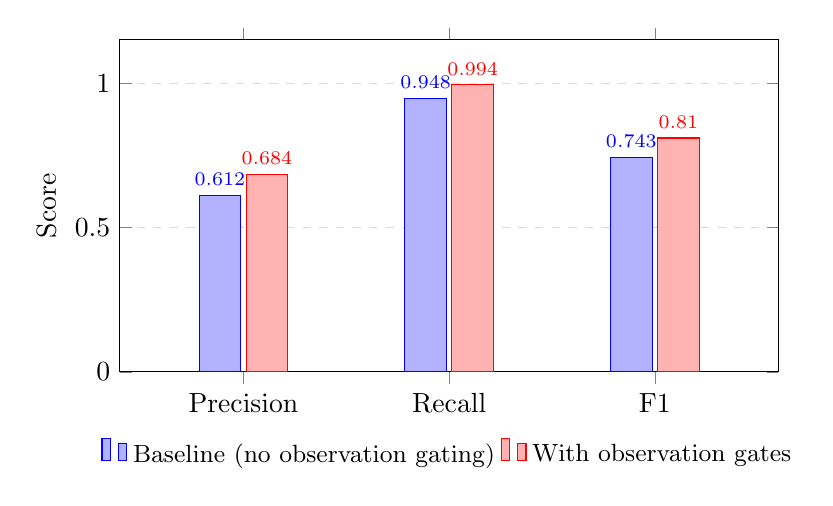
\begin{tikzpicture}
\begin{axis}[
    ybar,
    width=0.82\textwidth,
    height=58mm,
    bar width=15pt,
    ymin=0, ymax=1.15,
    ylabel={Score},
    symbolic x coords={Precision, Recall, F1},
    xtick=data,
    nodes near coords,
    nodes near coords style={font=\scriptsize, /pgf/number format/fixed,
                             /pgf/number format/precision=3},
    legend style={at={(0.5,-0.18)}, anchor=north, legend columns=2, font=\small,
                  draw=none},
    enlarge x limits=0.3,
    ymajorgrids=true,
    grid style={dashed, gray!30},
]
\addplot coordinates {(Precision,0.612) (Recall,0.948) (F1,0.743)};
\addplot coordinates {(Precision,0.684) (Recall,0.994) (F1,0.810)};
\legend{Baseline (no observation gating), With observation gates}
\end{axis}
\end{tikzpicture}
\caption{Observation-gate ablation. Gating raises precision without sacrificing recall,
yielding the net $F_1$ gain.}
\label{fig:ablation}
\end{figure}

As Figure~\ref{fig:ablation} makes visible, observation gating raises $F_1$ by
$+0.067$ (from 0.743 to 0.810), driven by a
precision gain (numeric-precondition recommendations no longer fire for every CCD patient)
with recall essentially unchanged. Because both configurations
share the same baseline, the ablation isolates the contribution of observation gating
itself. What it does not isolate is the contribution of the container. Whether that gain
actually requires FHIR is a separate question, and it is tested on its own in
Section~\ref{sec:csv-gating}.

\subsection{Where the gain comes from}
\label{sec:ablation-class}
A single overall figure hides more than it shows, because most of what it averages
cannot move at all. Section~\ref{sec:disc-class} sorts the 68 non-contraindication
recommendations by how each one can narrow the cohort, and only the 15 that carry a numeric
precondition are scored any differently with gating switched on. The other 53 give the same
answer either way, so they dilute the average without contributing to the change it is meant
to show. Table~\ref{tab:ablation-class} therefore reports concordance for each class
separately, in both arms.

\begin{table}[h]
\centering
\caption{Concordance by discrimination class in both ablation arms, micro-averaged over
the 876-patient cohort. Classes are those of Section~\ref{sec:disc-class}:
\emph{universal} recommendations carry no mechanism for narrowing the cohort at all,
\emph{concept-matched} require a further condition target, \emph{value-gated} a numeric
predicate over an observation, and \emph{both} require the two together. The two ungated
classes are identical in both arms to the individual count; the entire ablation effect is
confined to the 15 gated recommendations.}
\label{tab:ablation-class}
\footnotesize
\setlength{\tabcolsep}{4pt}
\begin{tabular}{lr|ccc|ccc}
\hline
& & \multicolumn{3}{c|}{\textbf{Baseline (no gating)}}
  & \multicolumn{3}{c}{\textbf{With observation gates}} \\
\textbf{Class} & \textbf{recs} & \textbf{P} & \textbf{R} & \textbf{$F_1$}
                               & \textbf{P} & \textbf{R} & \textbf{$F_1$} \\
\hline
Universal        & 38 & 0.666 & 1.000 & 0.799 & 0.666 & 1.000 & 0.799 \\
Concept-matched  & 15 & 0.676 & 0.915 & 0.777 & 0.676 & 0.915 & 0.777 \\
Value-gated      & \phantom{0}5 & 0.194 & 1.000 & 0.325
                                & \textbf{1.000} & \textbf{1.000} & \textbf{1.000} \\
Both             & 10 & 0.038 & 0.006 & 0.011
                                & \textbf{1.000} & \textbf{1.000} & \textbf{1.000} \\
\hline
\textbf{All}     & 68 & 0.613 & 0.945 & 0.743 & 0.685 & 0.993 & 0.811 \\
\hline
\end{tabular}
\end{table}

Four results follow from Table~\ref{tab:ablation-class}.

First, the two ungated classes are \emph{identical} across the arms---not merely close, but
equal to the individual true-positive, false-positive and false-negative count
($22{,}158/11{,}130/0$ for universal, $2{,}018/969/188$ for concept-matched). Fifty-three of
the 68 recommendations are therefore untouched, and the whole of the reported $F_1$
difference originates in the remaining 15. This is a falsifiable prediction of the
classification in Section~\ref{sec:disc-class}, and it holds exactly.

Second, the two gated classes benefit in opposite ways. For the \emph{value-gated} five, gating is a \emph{precision} mechanism: without it they
fire for every cohort member (849 true positives against 3{,}531 false positives,
$P = 0.194$), and with it they fire only where the measured value satisfies the predicate
($P = 1.000$) while recall was already perfect. For the \emph{both} class, gating is overwhelmingly a \emph{recall} mechanism. In the
baseline arm these ten recommendations almost never fire at all (8 true positives against
1{,}263 false negatives, $R = 0.006$), because their encoded condition targets alone rarely
match. The observation predicate is what actually identifies the patients they apply to. Describing the ablation solely as a
precision improvement is therefore incorrect for two thirds of the affected
recommendations.

Third, both gated classes reach $P = R = 1.000$ once gating is switched on. That
perfect score says something about the plumbing, not about how hard the clinical judgement is.
The observation gate and the reference standard apply the same guideline thresholds, such as
an ejection fraction at or below 40\%. They read the patient's value from different places,
however. The gate reads it from the graph, and the reference standard from the raw FHIR
bundle. Agreeing on every patient therefore shows that the loader carried those values across
without altering them. It does not show that the thresholds are clinically right, because both
sides were given the same thresholds to start with. Section~\ref{sec:shared-predicate}
establishes that the two are in fact the same function, then measures how much of the
concordance figure rests on that.

Fourth, five of the ten \emph{both}-class recommendations are \emph{inert}. \texttt{TP:2},
\texttt{TP:3:1}, \texttt{TP:3:2}, \texttt{TP:4} and \texttt{TP:5} record zero true positives,
zero false positives and zero false negatives in \emph{both} arms, and so contribute nothing to
either column. All five gate on a single predicate---current daily smoking---which no patient in
the cohort satisfies: of the 876, 390 are recorded as never having
smoked, 237 as ex-smokers, 249 carry no smoking observation at all,
and 0 are current smokers. The \emph{both} row is therefore driven entirely by five
active recommendations, and the counts quoted above belong to those five rather than to ten.
\texttt{LIPID:9} is inert for the same kind of reason---no cohort patient meets its
conjunction---so the gate it acquired when triglycerides were loaded is never exercised.

This generalises beyond the gated classes. 22 of the 73 recommendation
identifiers in the reference-label file have no positive instance anywhere in the cohort. That is
a property of the synthetic population rather than of the encoding: the recommendations are
encoded correctly and would fire given the relevant patients. It nonetheless bounds what these
concordance figures can demonstrate, and a real cohort would exercise a different and probably
larger subset. Section~\ref{sec:module-yield} identifies the principal cause. Of the 876 patients, 249,
some 28\%, come from the disease-enriched Synthea run. Their records carry only an
ischemic-heart-disease diagnosis, an abnormal cardiac imaging finding and sometimes a bypass
history, with no comorbidity and, apart from ejection fraction, no observation at all.

One choice of averaging runs through the whole table. The figures are \emph{micro}-averaged: every true positive, false positive and false
negative in the cohort is added up first, and the ratios are computed once at the end.

The other option, \emph{macro}-averaging, scores each patient on their own and then averages
those scores. It does not work here. A patient may not be touched by a class at all. There is then nothing for the system to get
right and nothing for it to get wrong, so all three counts are zero. Precision, recall and
$F_1$ are set to zero in that case, rather than left blank. That zero
goes into the average as though the system had failed the patient. The rarer the class, the
more such patients there are, and the further its macro figure sinks. What the number ends up
measuring is how common the class is, not how well the system handled it.

The value-gated class shows this at full size: macro $F_1 = 0.600$ against a micro value of
$1.000$. The two do not contradict each other. Because that class has no false positive and no
false negative anywhere, every patient scores either exactly one or exactly zero, so the macro
figure is simply the fraction of the cohort carrying a value-gated recommendation at all---526
of the 876. Every patient the class does apply to is scored perfectly. That is why every
per-class figure reported here is micro-averaged.

\subsection{Which part an independent judge scored}
\label{sec:shared-predicate}
Section~\ref{sec:oracle} separates the reference standard's independence into two tiers. This
section reports what that does to the figures.

For the 15 observation-gated recommendations, the system's predicate and the reference
standard's rule are the same function. This was checked empirically rather than read off the
source: both sides were evaluated on the 876 real cohort feature vectors and on 200{,}000
synthetic vectors aimed at every threshold they test, missing values included, and not one of
the 200{,}876 comparisons differed. Precision and recall of $1.000$ in the two gated classes
therefore cannot be read as a verdict on whether the rule is right.

Table~\ref{tab:shared-predicate} separates the two.

\begin{table}[h]
\centering
\caption{Guideline concordance split by the tier of independence of its reference standard,
micro-averaged over the 876-patient cohort.}
\label{tab:shared-predicate}
\begin{tabular}{lrcccrrr}
\hline
\textbf{Subset} & \textbf{recs} & \textbf{Precision} & \textbf{Recall} & \textbf{$F_1$} &
\textbf{tp} & \textbf{fp} & \textbf{fn} \\
\hline
All                & 68 & 0.685 & 0.993 & 0.811 & 26{,}296 & 12{,}099 & 188 \\
Shared predicate   & 15 & 1.000 & 1.000 & 1.000 & 2{,}120 & 0 & 0 \\
Independent logic  & 53 & 0.666 & 0.992 & 0.797 & 24{,}176 & 12{,}099 & 188 \\
\hline
\end{tabular}
\end{table}

The part scored by a genuinely independent judge covers 53 of the 68 recommendations and reaches
precision $0.666$ and $F_1$ $0.797$. Removing the fifteen shared-predicate recommendations
therefore costs $0.018$ of precision and $0.013$ of $F_1$; $8.1\%$ of all true positives come
from the shared-predicate part. The headline figure is not propped up by the shared part, and
the concordance conclusion survives deleting that part entirely.

The ablation is a different matter, and should be stated frankly. Only the value-gated and both
classes change between the ablation arms, and those are exactly the fifteen shared-predicate
recommendations. The whole of the ablation gain is therefore measured on recommendations whose
reference standard applies the same rule as the system. The gain is still a real change in the system's behaviour. Ungated, numeric-precondition
recommendations fire for patients who do not meet the precondition the guideline states, and
that is a defect whoever judges it. What the gain measures, though, is implementation
fidelity, not clinical validity. The reference standard is an
independent judge of the values fed to the rule, not of the rule.

\subsection{Does the gain require FHIR?}
\label{sec:csv-gating}
The ablation in Table~\ref{tab:ablation} isolates the contribution of observation gating, not
the contribution of the container. The two are easily conflated. Chapter~I motivates the
FHIR-native design by contrast with flattened tabular exports, from which it is a short step to
concluding that the gate is possible \emph{because of} FHIR. That conclusion was asserted rather
than measured. This section measures it.

The test is a third arm. The same gate was rebuilt reading only Synthea's CSV
export---\texttt{observations.csv} and \texttt{conditions.csv}---touching neither the bundles nor
the graph. The string-matching logic, the thresholds and the aggregation rules were copied
verbatim from \texttt{silver\_oracle.py}, so that any disagreement would be attributable to the
container and not to a difference in clinical logic. That is the point of the design.

The comparison target is the FHIR bundle path, not the graph path. For this purpose they are the
same thing: the fifteen observation-gated recommendations score precision and recall of $1.000$
against the reference standard across the whole cohort, as reported in
Section~\ref{sec:ablation-class}, so the graph's gate decisions and the reference standard's
already agree everywhere. Reproducing the reference standard therefore reproduces the graph gate
too, without needing Neo4j.

Table~\ref{tab:csv-gating} reports the result.

\begin{table}[h]
\centering
\caption{The observation gate built from the FHIR bundles against the same gate built from the
CSV export, for the 15 observation-gated recommendations across 876 patients.}
\label{tab:csv-gating}
\begin{tabular}{lcccrrr}
\hline
\textbf{Source} & \textbf{Precision} & \textbf{Recall} & \textbf{$F_1$} &
\textbf{tp} & \textbf{fp} & \textbf{fn} \\
\hline
FHIR bundles & 1.000 & 1.000 & 1.000 & 2{,}120 & 0 & 0 \\
CSV export   & 1.000 & 1.000 & 1.000 & 2{,}120 & 0 & 0 \\
\hline
\end{tabular}
\end{table}

Of 13{,}140 gate decisions---876 patients times 15 recommendations---not one differs between the
two sources. The count of 2{,}120 is itself the sum of the true positives of the two gated
classes in the gated arm of Table~\ref{tab:ablation-class}---849 for value-gated and 1{,}271 for
both---so the agreement doubles as a check that the reconstruction measures the same thing. The
cohort fares likewise: SNOMED~CT code \texttt{414545008} in \texttt{conditions.csv} selects
exactly the same 876 patients as the graph's gate.

Two things the export genuinely loses can be measured, and neither changed a decision. First,
the export rounds observation values to one decimal place. That makes 1{,}990 values differ
between the two paths, by at most $0.05$. Three of them land on the far side of a threshold. One
ejection-fraction case ($39.999$ becoming $40.0$) is not exposure at all, because the predicates
that use it test ``$\le 40$'' and ``$> 40$'', which both values answer identically. Two triglyceride cases ($149.97$ and $149.96$, both becoming $150.0$) are real exposure,
because the clause ``$150 \le$ triglycerides'' flips to true. \texttt{LIPID:9}, however,
also requires LDL below 100, which fails for both patients ($130.1$ and $148.6$). No recommendation changed.

Second, the blood-pressure panel does not survive, exactly as Section~\ref{sec:flattening} states.
Recovering it, however, requires no guesswork. The \texttt{ENCOUNTER} column is populated on every
observation row, so the 17{,}177 systolic and diastolic pairs in this cohort reassemble completely,
leaving no row unpaired. The reassembly is a cost, not an obstacle.

The conclusion that follows is narrower than Chapter~I originally asserted. The precision gain is
real and unchanged: observation gating still raises $F_1$ by $+0.067$. What the evidence does not
support is attributing that gain to the FHIR container specifically. What produces it is loading
numeric observation values as first-class data. FHIR makes that direct; Synthea's tabular export
permits it too, at the price of one reassembly step and one decimal place of precision. The distinction matters because it sets what may be claimed. The claim is not that FHIR is
necessary, but that numeric observations are. FHIR is the most direct way to obtain them.

The scope of this conclusion should be stated plainly. What the test shows is that Synthea's CSV
export carries enough data for the nine LOINC codes this gate uses, on this corpus. It does not
show that CSV and FHIR are equivalent in general, and it does not extend to tabular exports from
other systems, which need not carry a foreign key such as \texttt{ENCOUNTER}. The things the
export does still lose---resource \texttt{status}, the code system on an observation value, and
the panel's identity as a unit---are discussed in Section~\ref{sec:flattening}; none is used by
this gate, but that is a property of this corpus rather than of the design.

\section{Silver-Standard Validation Against the Gold Standard}
\label{sec:gold}

To validate the automatically generated silver standard, 30 patients were
labelled manually to form the gold standard and compared against the silver labels.
Agreement was 99.5\% (2{,}150 of 2{,}160 cells) with Cohen's
$\kappa = 0.991$ (95\% confidence interval 0.984--0.996; Section~\ref{sec:kappa-ci}),
indicating near-perfect agreement. This is the result that
licenses the rest of the evaluation. Because the silver standard reproduces human
judgement almost exactly on the sample where both exist, the concordance figures computed
against it over the full 876-patient cohort rest on a validated reference
rather than an assumed one. That is the standard justification for substituting
automatically generated labels for manual annotation at scale
\cite{rebholz2011,nogues2022}. The annotator and the rubric are given in Section~\ref{sec:goldlabel}.

\subsection{The residual disagreements}
Ten of the 2{,}160 compared cells disagree. They are enumerated individually in
Table~\ref{tab:disagreements} rather than summarised, because their distribution is more
informative than their count.

\begin{table}[h]
\centering
\caption{All silver--gold disagreements. ``Over'' denotes the silver standard labelling a
recommendation applicable where the human did not; ``under'' the reverse.}
\label{tab:disagreements}
\footnotesize
\begin{tabular}{llccl}
\hline
\textbf{Patient} & \textbf{Recommendation} & \textbf{COR} & \textbf{Silver / Gold}
& \textbf{Direction} \\
\hline
\texttt{cbf432fc} & \texttt{APT:6}    & 2b & 1 / 0 & over  \\
\texttt{6595b70f} & \texttt{BB:2}     & 1  & 0 / 1 & under \\
\texttt{1db4196c} & \texttt{BPM:3}    & 1  & 1 / 0 & over  \\
\texttt{05e41fe3} & \texttt{LIPID:2}  & 1  & 1 / 0 & over  \\
\texttt{22f599b6} & \texttt{LIPID:2}  & 1  & 1 / 0 & over  \\
\texttt{2b050f16} & \texttt{LIPID:2}  & 1  & 0 / 1 & under \\
\texttt{2b050f16} & \texttt{LIPID:3}  & 1  & 1 / 0 & over  \\
\texttt{04287b67} & \texttt{LIPID:5}  & 2a & 0 / 1 & under \\
\texttt{cbf432fc} & \texttt{LIPID:5}  & 2a & 0 / 1 & under \\
\texttt{227e76d8} & \texttt{LIPID:10} & 2b & 0 / 1 & under \\
\hline
\end{tabular}
\end{table}

Three properties of this set matter. First, the disagreements are \emph{exactly balanced}:
five over-labels and five under-labels, against 1{,}080 cells where both mark the
recommendation applicable and 1{,}070 where both do not. The silver standard is therefore
not systematically more or less permissive than the human labeller, which is the property
that most threatens the use of an automated reference and the one hardest to establish by
argument alone.

Second, the disagreements are \emph{concentrated}, not scattered: seven of the ten concern
lipid recommendations (\texttt{LIPID:2} three times, \texttt{LIPID:5} twice,
\texttt{LIPID:3} and \texttt{LIPID:10} once each). This is where the guideline text is
least mechanisable. \texttt{LIPID:2} applies when high-intensity statin therapy is
``contraindicated or not tolerated''---intolerance is not represented in the coded record,
so both the silver standard and the human must infer it. \texttt{LIPID:5} applies to
patients ``judged to be at very high risk'', a composite the guideline explicitly leaves
to clinical judgement. \texttt{LIPID:10} requires simultaneously that the patient is
\emph{not} at very high risk, is on ``maximally tolerated'' statin therapy, and has
LDL-C~$\geq$~70~mg/dL. These are precisely the clauses the reference standard's
unconfirmable-clause policy (Section~\ref{sec:oracle}) abstains on. The residual error is
therefore localised to irreducibly judgemental preconditions rather than distributed
across the recommendation set, which is the more reassuring of the two possibilities.

Third, the ten cells represent \emph{fewer than ten independent judgements}. Patient
\texttt{2b050f16} accounts for two of them---an under-label on \texttt{LIPID:2} and an
over-label on \texttt{LIPID:3}---which together are most plausibly a single disagreement
about statin intensity recorded in two cells; patient \texttt{cbf432fc} likewise accounts
for two. Cohen's $\kappa$ treats every cell as independent, so the reported value slightly
\emph{understates} the true level of agreement.

\subsection{Uncertainty of $\kappa$ and whether 30 patients suffice}
\label{sec:kappa-ci}
The same dependence bears on the uncertainty of $\kappa$. The 2{,}160 compared cells are
clustered in 30 patients, and one patient's record determines all of that patient's labels at
once. The appropriate confidence interval therefore resamples \emph{patients}, not cells
(Section~\ref{sec:goldlabel}). Table~\ref{tab:kappa-ci} reports both, so the difference can be
seen.

\begin{table}[h]
\centering
\caption{95\% confidence intervals for the silver--gold Cohen's $\kappa$, from 10{,}000
bootstrap replicates for each resampling unit.}
\label{tab:kappa-ci}
\begin{tabular}{lcc}
\hline
\textbf{Resampling unit} & \textbf{Lower bound} & \textbf{Upper bound} \\
\hline
Cells, assuming independence & 0.984 & 0.996 \\
Patients (cluster bootstrap)  & 0.984 & 0.996 \\
\hline
\end{tabular}
\end{table}

Both give the same interval, 0.984 to 0.996. The reason is how the disagreements are spread.
The ten disagreements fall on 8 of the 30 patients, and no patient contributes more than two.
The design effect is only 1.04, so clustering by patient adds almost no uncertainty. A
jackknife that drops one patient at a time gives $\kappa$ between 0.990 and 0.992. No single
patient, therefore, is holding the figure up.

Nor is $\kappa$ inflated by label prevalence. Positive labels cover 1{,}085 of 2{,}160 cells in
both standards (50.2\%), the prevalence index is 0.005, and the bias index is zero because the
disagreements split five and five. Chance agreement is therefore about 0.500, and $\kappa$ is
practically equal to PABAK, at 0.991 \cite{byrt1993}.

Whether 30 patients suffice depends on the claim being supported. For the claim that the silver
standard agrees near-perfectly with manual labelling, 30 patients are enough. The lower bound of
the interval, 0.984, is well above the 0.80 threshold \cite{landis1977}, and none of the 10{,}000
replicates falls below 0.95. For a finer claim, such as that $\kappa$ is 0.99 rather than 0.98,
30 patients are not enough, and no such claim is made.

The interval has two bounds. First, it describes only patients like these thirty, who were
chosen purposively and lean towards the most complex records (Section~\ref{sec:gate}). Second,
it does not address the single-annotator limitation, since resampling cannot produce a second
rater (Section~\ref{sec:limitations}).

\section{Safety Detection}
\label{sec:safety-detection}

Contraindication-safety detection was evaluated on the 151 manually labelled
safety flags (Table~\ref{tab:safety}).

\begin{table}[h]
\centering
\caption{Contraindication-safety detection: unary vs.\ population-gated matching.}
\label{tab:safety}
\begin{tabular}{lccc}
\hline
\textbf{Variant} & \textbf{Precision} & \textbf{Recall} & \textbf{$F_1$} \\
\hline
Unary (on the contraindicated drug) & 0.139 & $\approx$1.000 & --- \\
Population-gated (drug \emph{and} population condition) & 1.000 & 0.095 & 0.174 \\
\hline
\end{tabular}
\end{table}

The result exposes a genuine trade-off rather than a tunable failure: unary matching never
misses a reachable contraindication but over-flags heavily, whereas population gating is
perfectly precise but recovers only the minority of contraindications whose population
condition is structurally gateable; the misses are the negation-defined and conjunctive
contraindications that a flat schema cannot express.

Beyond this binary trade-off, the chronic-NSAID recommendation (\texttt{APT:10}) was scored
under a third, \emph{chronicity-gated} variant that fires only when the graph judges the
NSAID use chronic from the categorical medication status and the recurring-course count.
Against the manually labelled flags this variant reached precision 0.909 and
recall 0.526 (tp $=10$, fp $=1$, fn $=9$)---highly precise, but
recovering only about half of the truly chronic cases. The missed cases are precisely those that are chronic \emph{only} through a single long
course, for example a 101-day and a 111-day ibuprofen prescription. The graph cannot see
such cases because the FHIR export lacks stop dates (Section~\ref{sec:chronicity}). This is
not a tuning artefact but a measured price of the FHIR-native design: the categorical
medication status recovers the ongoing and multi-course arms of the chronicity rule, but the
duration arms are structurally unrecoverable from FHIR alone.

\section{Briefing Faithfulness}
\label{sec:faithfulness}

The grounded briefing was generated for 30 patients, the same sample as the gold standard,
and checked automatically against the retrieved facts. Five of them were generated first and
formed the basis of this work's initial report. The other twenty-five were generated later
with the same pipeline and model.

The check tests four things. First, every recommendation identifier the briefing cites must
be in the facts. Second, every PMID it cites must be in the facts too. Third, every
applicable recommendation and every safety flag in the facts must be mentioned. Fourth, the
briefing must not state that the patient requires oral anticoagulation when no anticoagulant
is on the medication list. A conditional statement such as ``if requiring oral
anticoagulation'' is still allowed.

All 30 briefings pass all four tests: zero fabricated recommendations, zero fabricated PMIDs,
zero omitted recommendations, and zero anticoagulation over-claims.

The fourth test needs to be reported with its history. On its first run over the 30
briefings, it flagged 10 lines in 4 briefings as over-claims. All 10 turned out to be false
positives of the same shape. The briefing's provenance trace wrote ``conditional on oral
anticoagulation need (not confirmed in current medications)'', and the pattern matched the
word \emph{on} inside \emph{conditional on}. The test was then restricted to the parts of the
briefing a reader acts on. Mentions in the provenance trace are still counted and reported,
not discarded. That correction was made \emph{after} the output was seen, and it should be
stated. The five-of-five result in the initial report held partly because the first five
briefings happened to phrase their conditional statements in a form the check recognised.

These four tests are not the same as semantic faithfulness. Deterministic retrieval
guarantees that the facts the language model receives are exact and reproducible. It also
makes citable items checkable against a closed set of facts. It does not, however, guarantee
that every sentence the model writes is faithful to those facts. The model can still, for
example, attach to the patient a condition or drug that is not in the facts, misstate why a
recommendation applies, or present a weak-class recommendation as if it were mandatory.
Apart from the anticoagulation pattern, none of these errors is caught by this check. What is
reported here is therefore citation-level and completeness faithfulness, plus one over-claim
pattern. The semantic faithfulness of every sentence still requires a human reading, and it
is recorded as a limitation in Section~\ref{sec:limitations}.

The briefing's safety tier applies the same graph-only chronicity gate as the recommendation
layer. For patients whose NSAID use is chronic \emph{only} by duration, the chronic-NSAID flag
is therefore withheld rather than asserted without support. That omission is consistent with
the safety-detection recall reported in Section~\ref{sec:safety-detection}, and traceable to
it.

Appendix~\ref{app:briefing} reproduces one briefing in full, unedited, so that what the check actually inspects can be read directly rather than described.

\section{Clinician Review}
\label{sec:clinician}

This section reports clinicians' judgements of the appropriateness of the recommendations the
system outputs (Section~\ref{sec:clinician-method}). Table~\ref{tab:clinician} summarises the
ratings by rater and by recommendation type. Antithrombotic recommendations cover
antiplatelet and anticoagulant therapy (\texttt{APT}); beta-blocker recommendations cover the
review of long-term use and the beta-blocker check/stop flags (\texttt{BB}).

\begin{table}[h]
\centering
\caption{Clinician ratings by rater and recommendation type. Percentages are of the rows that
rater rated.}
\label{tab:clinician}
\small
\begin{tabular}{llrrrr}
\hline
\textbf{Rater} & \textbf{Recommendations} & \textbf{Rows} & \textbf{Appropriate} &
\begin{tabular}[b]{@{}r@{}}\textbf{Not yet}\\\textbf{appropriate}\end{tabular} &
\begin{tabular}[b]{@{}r@{}}\textbf{Cannot be}\\\textbf{judged}\end{tabular} \\
\hline
A (cardiologist)  & Antithrombotic & 101 & 52  & 46 & 3  \\
                  & Beta blocker   & 40  & 35  & 5  & 0  \\
                  & Other          & 106 & 105 & 1  & 0  \\
                  & All            & 247 & 192 (77.7\%) & 52 (21.1\%) & 3 (1.2\%) \\
\hline
B (GP)            & Antithrombotic & 66  & 19  & 32 & 15 \\
                  & Beta blocker   & 25  & 9   & 1  & 15 \\
                  & Other          & 69  & 69  & 0  & 0  \\
                  & All            & 160 & 97 (60.6\%) & 33 (20.6\%) & 30 (18.8\%) \\
\hline
C (senior cardiologist) & All      & 16  & 6   & 5  & 5  \\
\hline
\end{tabular}
\end{table}

Rater~A judged 192 of 247 recommendations appropriate (77.7\%; 95\% per-patient confidence
interval 74.4--81.1\%). Rater~B judged 97 of 160 appropriate (60.6\%; 56.1--67.3\%). The
difference comes mostly from ``cannot be judged'', which rater~B chose on 30 rows and
rater~A on 3. Excluding those rows, the two proportions are closer, at 78.7\% and 74.6\%.

Judgements of inappropriateness concentrate on antithrombotic recommendations. Of the
``not yet appropriate'' ratings, 46 of rater~A's 52 and 32 of rater~B's 33 fall on them.
Outside the antithrombotic and beta-blocker recommendations, by contrast, rater~A judged 105
of 106 rows appropriate and rater~B all 69. That group covers the blood-pressure target and
first-line antihypertensives, cardiac-rehabilitation referral, weight management, SGLT2
inhibitors, and the safety flag for nitrates with a PDE5 inhibitor. It also includes three
shared-predicate recommendations (Section~\ref{sec:shared-predicate}): \texttt{WM:2},
\texttt{WM:3}, and \texttt{SGLT2:4}. All three were judged appropriate on all 30 of rater~A's
rows and all 20 of rater~B's. For those three, the clinicians' judgement provides a test of
the rule that the reference standard cannot.

Raters~A and~B both rated 159 rows across 10 patients. Their observed agreement is 65.4\%
(95\% per-patient confidence interval 58.8--73.9\%), with Cohen's $\kappa = 0.29$
(0.18--0.41) and PABAK 0.48. A $\kappa$ of that size is fair agreement \cite{landis1977}. The
agreement is uneven. On the 69 rows outside the antithrombotic and beta-blocker
recommendations, they agree on 68 (98.6\%). On the 90 antithrombotic and beta-blocker rows,
they agree on only 36 (40.0\%). Of the 55 disagreements, 27 involve rater~B's ``cannot be
judged''.

The raters' comments show where the disagreement comes from. Rater~A wrote none. Almost every
``cannot be judged'' from rater~B asks for information the conclusion did not show: ejection
fraction and heart-failure status for the beta-blocker recommendations, and bleeding risk for
extending dual antiplatelet therapy and for adding vorapaxar. On the three conditional
anticoagulant recommendations (\texttt{APT:11}--\texttt{APT:13}), rater~B chose ``not yet
appropriate'' on 23 of 24 rows. In their place, rater~B proposed a different sequence: triple therapy for one
week, then a DOAC with clopidogrel for up to one year, then a DOAC long term. Rater~A judged 13
of 15 clopidogrel check/stop flags (\texttt{APT:7}) not yet appropriate, and rater~B 5 of 11.
Rater~B's comments on those rows reject stopping clopidogrel: a post-infarction patient still
needs dual antiplatelet therapy, or clopidogrel alone if bleeding risk is high.

Rater~C judged 6 of the 16 recommendations for patient~1 appropriate. The comments expose a
limit of the review sheet. Rater~C chose ``cannot be judged'' for two check/stop flags,
clopidogrel and nitroglycerin, because neither drug appears in the conclusion, although both
are in the patient's record. The same option was given to the three conditional
anticoagulant recommendations, because the patient has no indication for anticoagulation.
Both beta-blocker check/stop flags were judged not yet appropriate, because in rater~C's view
the patient needs a beta blocker. On patient~1, rater~C agrees with rater~A on 6 of 16 rows
and with rater~B also on 6; all three agree on 5.

Overall, the clinicians judged most of the system's recommendations appropriate for their
patients. Rater~A, the cardiologist who rated the most patients (15), judged 77.7\%
appropriate. For rater~B, a general practitioner, the proportion judged appropriate is lower,
because more of rater~B's rows were marked ``cannot be judged''. Almost every recommendation
outside antithrombotic and beta-blocker therapy was judged appropriate, with high agreement
between the raters. By contrast, most ``not yet appropriate'' ratings fall on the
antithrombotic recommendations. On the beta-blocker recommendations, almost all the
disagreement between raters comes from ``cannot be judged''. Rater~B added that information
on ejection fraction and heart-failure status is needed for those recommendations to be
judged. The antithrombotic and beta-blocker recommendations therefore show a common pattern
in the ratings: they depend on information the system's conclusion did not present, such as
time since an acute coronary syndrome, bleeding risk, the indication for anticoagulation,
ejection fraction, and heart-failure status. The review thus shows that clinicians generally
judge the system's recommendations appropriate. It also identifies what to improve first: the
antithrombotic and beta-blocker recommendations, with an explanation of the information they
rest on.

\section{Comparison with Prior Work}
\label{sec:prior-work}

This section positions the results against previously published systems.
Table~\ref{tab:prior-systems} compares along the five dimensions that distinguish this
work: the data source, whether terminologies are bridged into a common concept space,
whether a clinical guideline is encoded as a queryable layer, whether the output is
evaluated against an independent reference, and whether generated text is mechanically
checked for faithfulness.

\begin{table}[h]
\centering
\caption{Comparison with prior knowledge-graph and FHIR-based clinical decision support.}
\label{tab:prior-systems}
\footnotesize
\setlength{\tabcolsep}{3pt}
\begin{tabular}{p{22mm}p{20mm}p{18mm}p{18mm}p{24mm}p{16mm}}
\hline
\textbf{Work} & \textbf{Data source} & \textbf{Concept bridge} & \textbf{Guideline layer}
& \textbf{Evaluated vs.\ reference} & \textbf{Faithful. checked} \\
\hline
This work
  & Synthetic FHIR R4 (Synthea)
  & UMLS CUI
  & 2023 AHA/ACC CCD, 81 recs
  & Independent oracle + manual gold ($\kappa$)
  & Yes, automated \\
Zhou \textit{et al.} \cite{zhou2022}
  & 124 records, one physician
  & Not reported
  & Chinese hypertension guideline
  & Ranking (recall, hit@3, MRR)
  & N/A (no text) \\
Semenov \textit{et al.} \cite{semenov2018}
  & FHIR engine, lab results
  & LOINC only
  & Production rules
  & Not reported
  & No \\
Xiao \textit{et al.} \cite{xiao2022}
  & OMOP CDM / MIMIC-III $\rightarrow$ FHIR RDF
  & OMOP vocab.
  & None
  & Query-equiv.\ + spec conformance
  & N/A (no text) \\
Cui \textit{et al.} \cite{cui2025}
  & Guideline text only
  & Ontology
  & Cardiovascular medication guides
  & Expert iterative review
  & N/A (no text) \\
Ehtesham \textit{et al.} \cite{ehtesham2025}
  & Synthetic FHIR R4 (SMART)
  & No
  & None
  & Not reported
  & No \\
Sudri \textit{et al.} \cite{sudri2024}
  & Angiography case notes
  & No
  & Implicit in model
  & Heart team, $\kappa = 0.59$
  & No \\
\hline
\end{tabular}

\vspace{2pt}
\end{table}

The closest system in capability is that of Zhou \textit{et al.}~\cite{zhou2022}, which
likewise couples a guideline-derived graph to patient records and evaluates the
recommendations it produces; Section~\ref{sec:rw-kg} sets out what separates the two.
The closest \emph{architectural} comparable is the FHIR-based patient decision aid of Semenov
\textit{et al.}~\cite{semenov2018}, which likewise pairs a FHIR interoperability layer with
a graph-structured knowledge base. It is, however, a production-rule system
over laboratory results, with a knowledge base of 365 test-component nodes,
5{,}084 rule nodes, and 49{,}932 connections. The graph
reported here is larger by more than two orders of magnitude in both nodes
(1{,}804{,}379 against roughly $5.4\times10^{3}$) and relationships
(8{,}796{,}425 against $4.99\times10^{4}$). The difference is one of
\emph{scope}, not of merit: that system encodes rules over a narrow laboratory panel,
whereas this one ingests entire longitudinal patient records.

On graph construction, Xiao \textit{et al.}~\cite{xiao2022} is the closest prior effort in
methodological rigour, exposing an OMOP repository as FHIR RDF and validating it by
query equivalence against the source database. Their MIMIC-III derived graph
is larger in patient count (46{,}520 patients against 5{,}490 here) because
it draws on a real intensive care corpus. Crucially, that work appears to stop
at the clinical graph: it reports no guideline layer and issues no
recommendations, so no concordance evaluation is possible. Conversely, Cui
\textit{et al.}~\cite{cui2025} build a cardiovascular medication guideline graph---also in
Neo4j, with 22{,}475 medication entities and 3{,}304
relationships---but with no patient records attached, so it supports
knowledge retrieval rather than patient-specific decision support. The contribution here is
precisely the join these two leave open: patient records and guideline recommendations in
one graph, bridged through shared concepts, with the patient-to-recommendation traversal
evaluated end-to-end. A related knowledge-graph analysis of stress echocardiography in
coronary disease~\cite{wu2023} is domain-adjacent but appears to be
a literature-mining study rather than a patient-facing system.

Two comparisons concern the language-model tier. Ehtesham \textit{et al.}~\cite{ehtesham2025}
also drive an LLM over synthetic FHIR records, but retrieval is agent-directed
rather than deterministic, and no faithfulness verification is reported---the property this
work treats as central. Sudri \textit{et al.}~\cite{sudri2024} work in the same clinical
territory (coronary revascularization) and report that an ungrounded GPT-4 reaches accuracy
0.82 and $\kappa = 0.59$ against a multidisciplinary heart
team, with GPT-3.5 at $\kappa = 0.12$.
\textbf{That figure is not directly comparable to the $\kappa = 0.991$ reported
in Section~\ref{sec:gold}}: theirs measures a language model's clinical judgement against
expert clinicians, whereas the value here measures an automated oracle against manual gold
labels. The relevant contrast is architectural rather than numerical---it indicates the
level of agreement obtainable when a model is asked to reason clinically without grounding,
which is the design this work deliberately avoids.

\subsection{Faithfulness in context}

The faithfulness result is best read against the framework of Asgari
\textit{et al.}~\cite{asgari2025}, who annotated 12{,}999 clinician-reviewed
sentences from LLM-generated clinical notes and measured a 1.47\%
hallucination rate and a 3.45\% omission rate
(Table~\ref{tab:faithful-compare}).

\begin{table}[h]
\centering
\caption{Faithfulness of generated clinical text: this work in context.}
\label{tab:faithful-compare}
\footnotesize
\begin{tabular}{lccl}
\hline
\textbf{Study} & \textbf{Fabrication} & \textbf{Omission} & \textbf{Evaluation sample} \\
\hline
Asgari \textit{et al.} \cite{asgari2025}
  & 1.47\% & 3.45\%
  & 12{,}999 clinician-annotated sentences \\
This work
  & 0 & 0
  & 30 briefings, all cited items checked \\
\hline
\end{tabular}

\vspace{2pt}
\end{table}

The two differ widely in both unit and sample size: clinician-annotated sentences against
automatically checked briefings. They therefore cannot be set side by side directly. The
correct statement about the briefings produced here is that \emph{no} fabrication or omission
was observed across 30 briefings whose cited items were all checked---not that this system
has a lower hallucination rate than the published benchmark. What the comparison does support is a claim about mechanism. Asgari
\textit{et al.} reduce errors by refining prompts and workflows, leaving a non-zero residual
because the model is still composing content. Here new citable content cannot get through
undetected: every citable item in the briefing must correspond to a retrieved fact, and the
check is decidable precisely because retrieval is deterministic. The residual risk therefore
shifts from fabrication to \emph{phrasing}. The over-claim check reaches only one pattern of
that risk (Section~\ref{sec:faithfulness}). Finally, the reader-study protocol of Van Veen \textit{et al.}~\cite{vanveen2023} had
physicians score summaries for completeness, correctness, and conciseness. That evaluation
is not performed in this work, since the clinician review of Section~\ref{sec:clinician}
judges the appropriateness of recommendations, not the quality of the summary. Faithfulness here is established against the record rather
than against a clinician's judgement, and closing that gap is the reader study proposed in
Section~\ref{sec:limitations}.

\section{Discussion}

Taken together, the results support the three research questions. First, a FHIR-native
knowledge graph fusing EHR, guideline, and literature was constructed and shown to be rich,
broad, and deeply connected. Second, loading numeric observations as first-class data
improved guideline concordance by $+0.067$ $F_1$ without loss of recall. FHIR supplies those
observations most directly, but not uniquely, since a tabular export reproduces the same gate
(Section~\ref{sec:csv-gating}). Third, all 30 grounded briefings passed the automated
faithfulness check. Because retrieval is deterministic, citable items can be checked against a
closed set of facts, which similarity-based retrieval-augmented generation cannot offer. That
advantage concerns citation-level faithfulness, not a guarantee that every sentence is
semantically faithful (Section~\ref{sec:faithfulness}). As
Section~\ref{sec:prior-work} sets out, prior FHIR-based graphs stop short of a guideline
layer \cite{xiao2022} while prior guideline graphs carry no patient records
\cite{cui2025}; joining the two and evaluating the join end-to-end is where this work sits.

The residual errors are honest and instructive. Guideline preconditions that structured
data cannot confirm (composite risk scores, some negation-defined clauses) remain sources of
false positives, and the safety tier makes the unary-vs-gated trade-off explicit. The
clinician review points to the same place from another direction. Outside the antithrombotic
and beta-blocker recommendations, clinicians judged almost every recommendation appropriate.
The ratings of inappropriateness, and the disagreement between raters, concentrate on
recommendations whose guideline logic depends on information outside the conclusion: time
since an acute coronary syndrome, bleeding risk, the indication for anticoagulation, ejection
fraction, and heart-failure status (Section~\ref{sec:clinician}). Some of that information,
such as bleeding risk, is a composite score that structured data cannot confirm. Some, such
as the medication list, is in the record but was not presented in the conclusion the
clinicians read. A further finding concerns interoperability. The synthetic FHIR export is SNOMED-native and, unlike the
paired CSV export, omits medication stop dates while retaining a categorical medication
status; the CSV, conversely, retains stop dates but carries no status. Neither projection is
a superset of the other, so the graph-side chronicity gate can reconstruct only two of the
four arms of the chronic-use rule (Section~\ref{sec:chronicity}). The cost of this loss is
measured, not hypothetical: the chronicity-gated safety variant recovers only
53\% of truly chronic NSAID courses (Section~\ref{sec:safety-detection}), and the
corresponding briefing flag is honestly withheld for the two patients whose chronicity is
duration-only. A real deployment that consumes only FHIR must anticipate this class of
information loss and, where a guideline depends on exposure duration, recover it from an
auxiliary source.
